% !TeX spellcheck = en_GB
% THIS IS SIGPROC-SP.TEX - VERSION 3.1
% WORKS WITH V3.2SP OF ACM_PROC_ARTICLE-SP.CLS
% APRIL 2009
%
% It is an example file showing how to use the 'acm_proc_article-sp.cls' V3.2SP
% LaTeX2e document class file for Conference Proceedings submissions.
% ----------------------------------------------------------------------------------------------------------------
% This .tex file (and associated .cls V3.2SP) *DOES NOT* produce:
%       1) The Permission Statement
%       2) The Conference (location) Info information
%       3) The Copyright Line with ACM data
%       4) Page numbering
% ---------------------------------------------------------------------------------------------------------------
% It is an example which *does* use the .bib file (from which the .bbl file
% is produced).
% REMEMBER HOWEVER: After having produced the .bbl file,
% and prior to final submission,
% you need to 'insert'  your .bbl file into your source .tex file so as to provide
% ONE 'self-contained' source file.
%
% Questions regarding SIGS should be sent to
% Adrienne Griscti ---> griscti@acm.org
%
% Questions/suggestions regarding the guidelines, .tex and .cls files, etc. to
% Gerald Murray ---> murray@hq.acm.org
%
% For tracking purposes - this is V3.1SP - APRIL 2009

\documentclass{acm_proc_article-sp-copy}

\begin{document}
	
\title{Automatically Deploy Deep Learning Models on FPGA}
%\title{F-TensorFlow: Automatically Deploying TensorFlow Described Deep Learning Models on FPGA with High Performance}

%\subtitle{[Extended Abstract]
%\titlenote{A full version of this paper is available as
%\textit{Author's Guide to Preparing ACM SIG Proceedings Using
%\LaTeX$2_\epsilon$\ and BibTeX} at
%\texttt{www.acm.org/eaddress.htm}}}
%
% You need the command \numberofauthors to handle the 'placement
% and alignment' of the authors beneath the title.
%
% For aesthetic reasons, we recommend 'three authors at a time'
% i.e. three 'name/affiliation blocks' be placed beneath the title.
%
% NOTE: You are NOT restricted in how many 'rows' of
% "name/affiliations" may appear. We just ask that you restrict
% the number of 'columns' to three.
%
% Because of the available 'opening page real-estate'
% we ask you to refrain from putting more than six authors
% (two rows with three columns) beneath the article title.
% More than six makes the first-page appear very cluttered indeed.
%
% Use the \alignauthor commands to handle the names
% and affiliations for an 'aesthetic maximum' of six authors.
% Add names, affiliations, addresses for
% the seventh etc. author(s) as the argument for the
% \additionalauthors command.
% These 'additional authors' will be output/set for you
% without further effort on your part as the last section in
% the body of your article BEFORE References or any Appendices.

%\numberofauthors{8} %  in this sample file, there are a *total*
% of EIGHT authors. SIX appear on the 'first-page' (for formatting
% reasons) and the remaining two appear in the \additionalauthors section.
%

% Just remember to make sure that the TOTAL number of authors
% is the number that will appear on the first page PLUS the
% number that will appear in the \additionalauthors section.
\toappearbox{djdjd}
\maketitle
\begin{abstract}
Deep learning has demonstrated great success in numerous applications such as image classification, speech recognition, video analysis, etc. However, deep learning models are much more computation-intensive and memory-intensive than previous shallow models, which makes their serving in large-scale data centers and real-time embedded systems big challenges. Considering performance, flexibility and energy-efficiency, FPGA-based accelerator for deep learning models is a promising solution. Unfortunately, conventional accelerator design flows make it hard for FPGA developers to keep up with the fast pace of innovations in deep learning.

In this paper, we propose an end-to-end framework that takes symbolic descriptions (TensorFlow in this work) of deep learning models as input, and automatically generates the hardware implementations on FPGA boards. We take an OpenCL HLS-based approach, and perform deep learning model inference with general-purpose computing kernels like GEMM, GEMV, etc. The framework automatically estimates the performance and resource utilization with the help of our proposed models, then chooses the optimal hardware configuration. Besides, we carefully design the processing units and data layout strategies for further optimizations. To show the great effectiveness and state-of-the-art performance provided by our proposed framework, we implement ANNs, CNNs and RNNs as our case studies.
\end{abstract}

% A category with the (minimum) three required fields
%\category{H.4}{Information Systems Applications}{Miscellaneous}
%A category including the fourth, optional field follows...
%\category{D.2.8}{Software Engineering}{Metrics}[complexity measures, performance measures]

%\terms{Theory}

\keywords{FPGA, TensorFlow, Compiler, Accelerator} % NOT required for Proceedings

\section{Introduction}
Deep learning models have raised a new storm of artificial intelligence, and achieved great improvements in several domains such as computer version[cite], speech recognition[cite], natural language processing[cite], etc. Inspired by the impressive breakthroughs achieved by deep learning models, many researchers in both academic and industry are studying in or integrating their work with powerful deep learning models. With their model accuracy closer to or even better than human, deep learning models are more and more deployed at scale in data centers by leading companies [Google translate APIs, Microsoft Cognitive Services], as well as in embedded systems like mobile phones and robots.

Deep learning models are well-known to be computation-intensive and memory-intensive because of their deep topological structures, complicated neural connections and massive data to process. These characteristics indicate that deploying pre-trained deep learning models with high performance and good energy efficiency becomes a big challenge. To solve this problem, many heterogeneous accelerators for deep learning model inference have been investigated recently. They are mainly based on GPU[cite], ASIC[cite] and FPGA [cite]. Among these designs, FPGA-based accelerators received great popularity with their strong flexibility and good energy efficiency.

Unfortunately, hand-coded FPGA-based accelerator faces both productivity and programmability challenges for deploying deep learning models in real applications. On the one hand, the design and optimization work of FPGA-based accelerator is quite heavy, which will typically cost a single professional hardware developer several weeks to migrate a deep learning model onto FPGA, even with the help of high-level synthesis tools. For deep learning model designers, there is no programming interfaces or libraries (like cuBLAS[cite?] and cuDNN[cite?] in Nvidia GPUs)  to easily and fast migrate their model to FPGAs. On the other hand, prior work on FPGA-based accelerator for deep learning models focus on accelerating certain type of layers[cite] or certain models[cite]. Since deep learning evolves rapidly, various model configurations and optimization techniques are emerging so fast that re-designing FPGA-based accelerator for every new model or technique is quite clumsy and inefficient.

According to the analysis above, there is a strong demand for an easy-to-use framework which can fast migrate deep learning models to FPGA implementations. In this paper, we propose a framework which takes symbolic descriptions (using TensorFlow) of deep learning models as input, and outputs implementations of the corresponding FPGA-based accelerators for model inference. The accelerators are implemented by OpenCL-based HLS, and we convert model inference into general-purpose computations like GEMM, GEMV, etc. Several performance and resource models are developed and invoked to ensure the functionality, performance and energy efficiency of the implemented accelerator. The whole compilation procedure is end-to-end and automated, which makes it possible for all deep learning researchers and users to use FPGA as a common device to perform model inference.

We make the following contributions in this paper:
\begin{itemize}
\item We offer a thorough analysis of factors affecting the performace on each function of DNN and propose the optimal solution on FPGA.
\item We build a framework which compiles deep learning models described in TensorFlow to FPGA implementation for model inference, and we test it with ANNs, CNNs and RNNs. Compared with previous accelerating work, this automated framework can save XXx design time on average. 
\item We implement high-performance matrix multiplication kernels for model inference, and carefully design the data layout strategies for further optimization. Several estimation models for performance and resource utilization are proposed, and our framework takes advantage of these models to explore the whole design space, and choose the optimal configuration as the final implementation.
\item We implement several deep learning models as case studies. The experimental results shows that our symbolic compiler offers great effectiveness, and the final FPGA-based accelerators show state-of-the-art performance and energy efficiency.
\end{itemize}

The rest of this paper is organized as follows: Section 2 introduces some basis of deep learning models, TensorFlow and OpenCL-based HLS. Section 3 describes detailed architecture of our proposed framework, then the hardware implementation and design space exploration are introduced in Section 4. In Section 5, we show the experimental setup and results of our case studies. At last, Section 6 concludes this paper and discusses about future work.

\section{Background}
In this section, we first introduce the characteristics of deep learning model inference, and the corresponding difficulties in hardware implementation. Then we provide some basis for TensorFlow and OpenCl-based HLS architecture.

\subsection{Deep Learning models}
Deep learning has evolved into a big community, and many interesting and powerful models have been proposed. These models can be divided into several categories. By topological structure, we can divide these models into Feed-Forward Neural Networks (FFNNs), Convolutional Neural Networks (CNNs), Recurrent Neural Networks (RNNs), etc [Figure?]. All these models are comprised of several neural layers. By types of layers, we can have fully-connected layers, convolution layers, recurrent layers, pooling layers, activation layers, etc. A single deep learning model can choose any topological structure mentioned above, and it may includes several types of layers in its configuration. So this results in a huge design space of possible model configurations.

The great flexibility and diversity of deep learning model configuration is indeed good to inspire more powerful models and designs, while it is a nightmare for hardware developers who accelerating certain type of layers or models. For example, convolution layers are well-known to be computation-intensive, while fully-connected layers and recurrent layers are memory-intensive. Pooling layers and different activation layers needs additional operations and hardware modules. Besides, every time the model configuration changes, the hardware developers have to work hard to modify or even re-design their implementations. 

\subsection{Tensorflow}
place holder for tf.
%TensorFlow [cite] is an open-source framework designed for deep learning as well as other scientific research, which is recently released and widely discussed about. Compared with previous deep learning frameworks (Caffe, mxnet,[cite]), TensorFlow is more like a programming library , and can support much more types of deep learning models. The programming model of TensorFlow in a symbolic style[cite]. Figure \ref{tf}(a) shows an example of a convolution layer described in TensorFlow. All the computations described in TensorFlow can be transformed into a computation graph (Figure \ref{tf}(b)), with each node in this graph representing a computation operation or a certain function. Data are viewed as tensors which stream across each node to get the final results of the whole computation. 
%We choose TensorFlow as our high-level description of deep learning models for the following reasons: First, it is programmed in Python and C++, and it also provides many APIs for developers, which makes it quite powerful and friendly to deep learning researchers. Second, it is popular and more flexible. It can support much more possibilities of model configuration (FFNN/CNN/RNN/...) when compared with other deep learning frameworks like Caffe (CNN only?). Last, the symbolic programming style is quite similar to the operations done in FPGA implementations (shown in Figure \ref{tf}(c)). The reconfigurable fabric is just like the computation graph in TensorFlow, and each hardware module can correspond to a node. Data to be processed are fed into FPGA, then the programmed logic ``cooks'' them to get the final results. This great similarity can help us a lot with the hardware implementations.

\begin{figure}
	\centering
	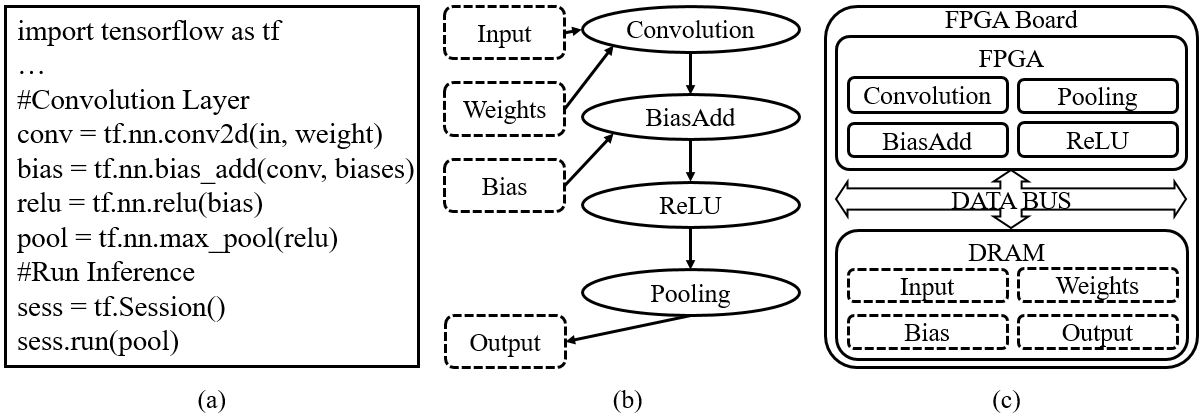
\includegraphics[width=1.0\linewidth]{./figure/tf.jpg}
	\caption{Comparison between TensorFlow and FPGA Implementation}
	\label{tf}
\end{figure}

\subsection{OpenCL-based HLS}
It is well-known that using hardware description languages (e.g. Verilog, VHDL) to design FPGAs is quite hard and time-consuming. Besides, the learning curve for beginners in hardware development is very steep. These two reasons make hardware design a heavy work for researchers. Fortunately, high-level-synthesis (HLS) tools help us solve this difficult problem. These tools receive designs programmed by high-level programming languages (C, C++, OpenCL, etc.), then transform them into the corresponding HDL descriptions and get the the final hardware configuration files. Among these tools, OpenCL-based HLS tool wins great popularity due to its flexible framework and great portability. Figure \ref{OpenCL-HLS} shows a rough framework of the FPGA implementations designed by OpenCL-based HLS. Similar to other OpenCL-based frameworks, the whole system is comprised of two main parts: $Host$ and $Device$. $Host$ is a desktop computer or server, where a C/C++ program is compiled and executed to perform the controlling operations. $Device$ is an FPGA board, which is plugged into the motherboard of $Host$ through a PCI-e slot. Data communication between $Host$ and $Device$c are accomplished through this PCI-e slot, and this slot is also used to power and program FPGA. Inside FPGA, hardware modules are compiled and invoked by $Host$ to complete the main computation tasks.

\begin{figure}
\centering
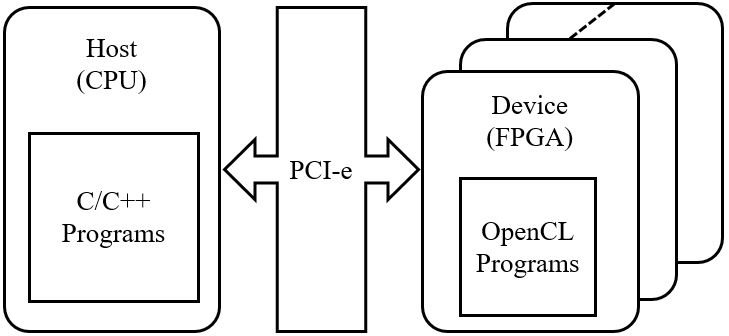
\includegraphics[width=1.0\linewidth]{./figure/OpenCL-HLS.jpg}
\caption{OpenCL-HLS Framework}
\label{OpenCL-HLS}
\end{figure}

\section{Framework}
We introduce the architecture of our proposed framework in this section. We first give an overview, then discuss about the main parts of it separately.

An overview of our overall framework is shown in Figure \ref{framework}. The whole framework is comprised of three parts: {\em Symbolic Compiler}, {\em Host Program}, and {\em Hardware Template}.

{\em Symbolic Compiler} takes symbolic descriptions of deep learning models (similar to TensorFlow) as input. It analysis the model and decide certain implementation-related parameters. After the analysis, S.C. uses these parameter to: 1) Instantiate hardware template and generate synthesizable hardware description. 2) Generate behavior script for {\em Host Program} to execute.

{\em Hardware Template} is a set of elaborately designed OpenCL kernels to implement different DNN functions. They are designed model-agnostic, thus could be flexablely reconfigured.

{\em Host Program} is a C++ program that serves the driver of hardware accelator. It takes {\em Symbolic Compiler} generated behavoir script as instruction.

The whole framework works in an ``end-to-end'' manner: from software-based model descriptions (TensorFlow codes) to FPGA-based model inference implementations (FPGA programming files), and this procedure is all done automatically without any human intervention.

\begin{figure}
	\centering
	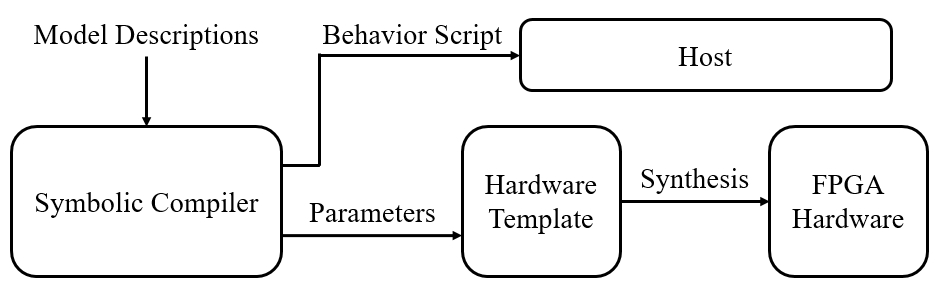
\includegraphics[width=1.0\linewidth]{./figure/z/framework.png}
	\caption{Overall Framework}
	\label{framework}
\end{figure}

\section{Symbolic Compiler}
Symbolic Compiler serve the role to map arbitary user defined network logic to certain hardware units. Network function are expressed by instructions on how hardware operates. 

Lets use a fraction of Microsoft Research 152 layer image net as a example to show the compiler work flow. 152 layer CNN is a very large network, still it has considerable local structure similariy: the main body of the network is composed by repeating certain kinds of structures, a) in Figure \ref{cflow} is one of these structures.

1) S.C. takes the U.S.E. and merges Element Wise Add layer into Convolution layer. It generates the data flow graph connect by execution units (OpenCL kernel) and storage units (DDR memory). Note an execution unit and its output storage units is one-one correspondence. For 152 layer network, there are exactly 152 (execution unit, storage unit) pairs.

2) S.C. maps large number of logic executions unit and storage units to limited hardware function units and DDR regions. The S.C. adopts such strategy:
For execution units, S.C. generate only one instance for each type of execution unit at hardware, map all execution units of the same type to the corresponding instance. e.g. for a given CNN model, all pooling layers reuse the same hardware pooling kernel, with respective parameter at runtime.
For storage units, S.C. maps all storage units to limited number of memory buffers. We use the same graph coloring strategy as {\em register allocation} in compiler back end, to find the mininum number of memory buffer possible for safe mapping.
In detail, storage unit is regarded as variables, and memory buffer as register. Take data flow graph in Figure \ref{cflow} as example.

[Cite] has proved this problem could be abstracted to a graph coloring problem. This graph coloring problem is NP hard and serveral heuristic algorithm has been proposed to optimize it. We choose DSATUR [Cite] algorithm as the solver for this problem.

3) S.C. takes this local structure

Show in Figure \ref{cflow}.
The detailed structure and working flow of our $Symbolic\ Compiler$ are shown in Figure \ref{cflow}.
Unified Symbolic Expression (U.S.E.). U.S.E. describes the topological structure and functionality of the models to be

\begin{figure}
	\centering
	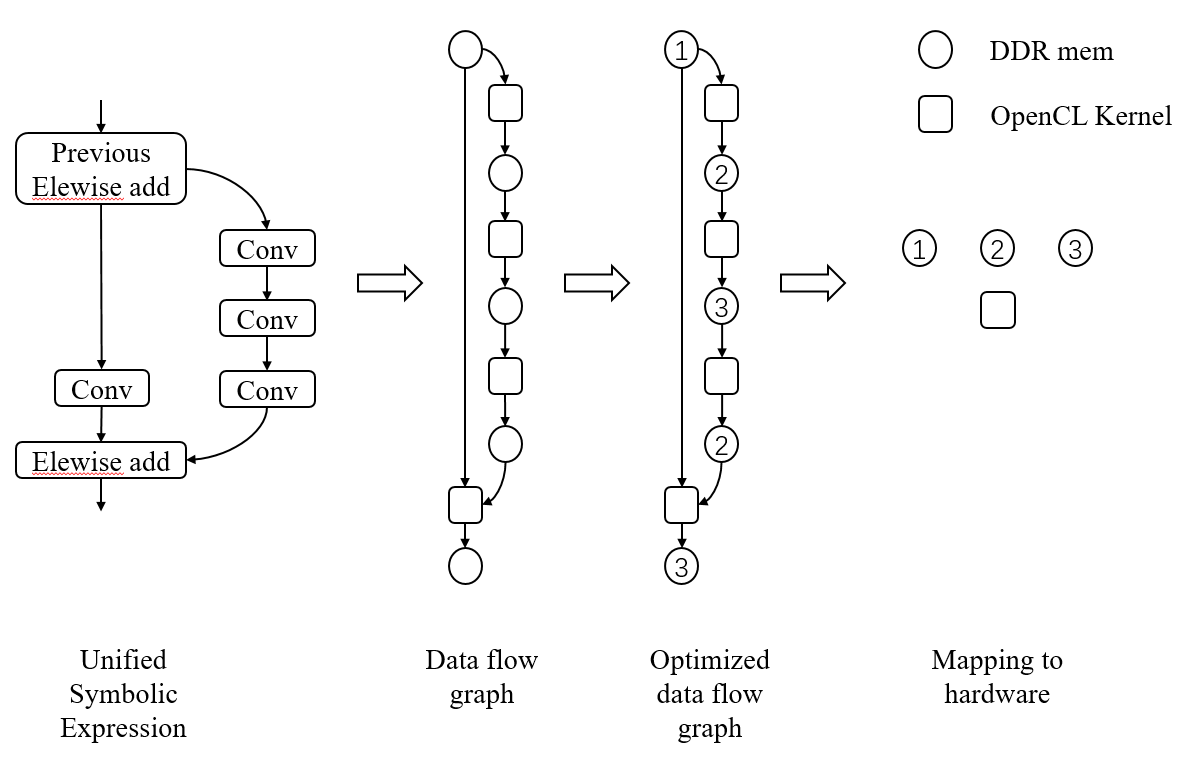
\includegraphics[width=1.0\linewidth]{./figure/z/compileflow.png}
	\caption{Compile Working Flow}
	\label{cflow}
\end{figure}

\section{Host Program}
Host program invokes OpenCL API.

\section{Hardware Template}
The complex structure and the great variaty of deep learning models has bring big challege to generate optimal hardware for them individually.
%To support various types of deep learning models in our framework, a unified computation kernel is strongly demanded.
We address this challenge by the observation that deep learning models share similar structure on computation intensive layers, which can always be expressed as $M\times M$ or $M\times V$.

We use a flexable General Purpose Matrix Multiplication (GEMM) engine to accerate the computing intensive part.
Our gemm is implemented using a tiling strategy, this strategy improves data locality, thus enables the slow DDR transfer to keep up with the high throughput computing.
In detail, the gemm is composed of three OpenCL kernels: $MM$, $Data_{in}$and $Data_{out}$.
$MM$ carries out the $tile \times tile$ task where the heavy computing lays.
$Data_{in}$ kernel devides a the matrix A and B into tiles and sends them to $MM$.
$Data_{out}$ receives the computing result as output tile from $MM$ and write it back to DDR.
Note that the matrix A, B, and C do not have to be stored in DDR as an actual matrix. $Data_{in}$ serves the role to virtualize matrices for $MM$, model specific logic and optimization are involved in this conversion process.
$Data_{in}$ and $Data_{out}$ kernel obey certain protocol on DDR data layout, to make sure $Data_{out}$ output reused for next round's $Data_{in}$.

%As a result, our approach is to seperate the computing intensive part and model specific logic part, and accelerate the computing intensive part with model-independent kernel $MM$, 
%we implement a scalable general purpose matrix multiplication (GEMM) kernel, and map each model's computation intensive part to it, we regard model specific logic as the order how data is feed to the GEMM kernel, and implement this data management kernel for each model seperately.
%Our GEMM is comprised of three OpenCL kernels: $MM$, $Data_{in}$and $Data_{out}$. $MM$ performs matrix multiplication, and details about it are provided in Section 4.1.
%$Data_{in}$ and $Data_{out}$ are data management kernels that convert input or output data into the format required by $MM$. All these kernels work in a single-workitem mode, which offers us more thorough control of the our kernels' behavior and performance.

We first give a detailed description about our gemm structure and performance model, then we give two cases in our project on how gemm accelerates specific tasks.

\subsection{GEMM details}
There are two fectors affecting gemm performance: IO bandwidth and computing power. In case of our experiment, matrix is stored in DDR3 memory and computing power is 1024 DSP.
\[ Bandwidth_{DDR} = 8GB/s \]
\[ Bandwidth_{comp} = 1024DSP \times 200MHz = 204.8 GB/s \]
This means IO can not keep up with computing in naive implementation. Our implementation solve this mismatch by exploring the data locality inside matrix multiplication. We fetch the matrix from DDR and buffer them on on chip block ram by tile. We configure block ram storage in a banked manner and feed data to computing units with high bandwidth. This strategy is shown in \ref{tile}.
%Since the size of matrices during deep learning model inference is usually too large to be processed all at once with the limited on-chip resource, we propose to perform these calculations in a tiling style, which is also the task of $MM$. Another advantage that the tiling strategy can bring is we can better explore the data locality, and improve the whole efficiency of matrices multiplication. Our tiling strategy can be generally shown in Figure \ref{tile}. The output matrix is tiled both in row and column, and the tiling size is denoted as $S_{tile}$. Then the two input matrices are tiled correspondingly to accomplish the matrix multiplication. To insure the computation are correctly performed in a tiling manner, we apply zero-padding to input matrices if any dimension of them is not divisible by its tiling size.

%\begin{figure}
%	\centering
%	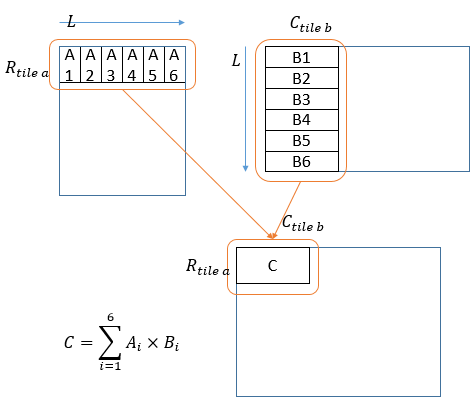
\includegraphics[height=2in, width=3in]{./figure/z/tile.png}
%	\caption{Tiling}
%	\label{tile}
%\end{figure}
\begin{figure}[h]
	\centering
	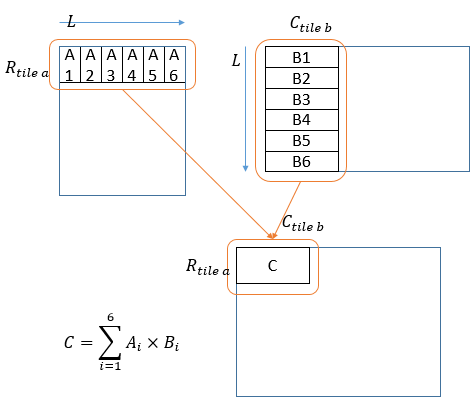
\includegraphics[width=1.0\linewidth]{figure/z/tile.png}
	\caption{Tiling}
	\label{tile}
\end{figure}

Figure \ref{mm} shows a general structure $Data_in$, $MM$, and $Data_out$. $MM$ takes in tile of matrix A and tile of matrix B from $Data_in$, and performs tile multiplying tile. We generate resuce tree hardware to perform $V\times V$. In practice, multiple sets of $V\times V$ hardware could be generate and work simultaneously to increase throughput, this configuration is update to the user's trade off between resource usage and performance.

Besides, we implement two set of buffers ($Buffer0$ and $Buffer1$ in Figure \ref{mm}). Each buffer the tiled input data, and they operate in a ping-pong manner: During a certain phase, $Dot\ Product\ Unit$ is processing with the tiles fetched from $Buffer0$, and the tiles to be processed in the next phase are loaded into $Buffer1$ simultaneously. Once $Dot\ Product\ Unit$ finished computing with current tiles, it comes to the next phase, and every operation reverses. $Dot\ Product\ Unit$ processes the tiles fetched from $Buffer1$, and $Buffer0$ loads the next tiles. In this manner, IO time consume could be hidden during computing.\\

In the tilig strategy, we use $R_{tile\_a}$ to denote row length of tile A, $C_{tile\_b}$ to denote column of tile B, $L$ to denote column of tile A and row of tile B. $L$ is also the vector dot product computing unit length. We use $N_{dot}$ to denote number of dot product units we generate. We use $thrIO$ to denote IO throught, which is proportional to the DDR bandwidth, $thrComp$ to denote computing unit throughput, which is proportional to the computing power we invest to $MM$ kernel (number of DSP). We have the following IO time consume and computing time consume comparasion:
\[ thrComp = L \times N_{dot} \]
\[ totalIO= R_{tile\_a} \times L + L \times C_{tile\_b} \]
\[ totalComp = R_{tile\_a} \times C_{tile\_b} \times L \]
\[ timeIO = totalIO / thrIO \]
\[ timeComp = totalComp / thrComp \]
Note in the ping-pong manner, we require $timeIO < timeComp$ to keep the computation unstalled. This condition equals:
\[ thrIO > thrComp \times (\frac{1}{R_{tile\_a}} + \frac{1}{C_{tile\_b}})\]
thrIO is FPGA board-specific and is always a constant. In our case it is 8GB/s, that is 64 8bit fix point numbers per cycle at 200MHz. This equision shows the following fact:
\begin{itemize}
\item Tile shape matters. For the certain bram resource ($R_{tile\_a} \times L$) to store a tile, the "narrower" tile shape we choose, the better data could be reused.
\item The more computing unit we employ, the bigger tile size is needed. This could be intuitively explained as the tile multiplication is $O(N^2)$ IO V.S. $O(N^3)$ computing, the bigger tile size we choose, the more we take advantage of this property.
\end{itemize}

\begin{figure}
	\centering
	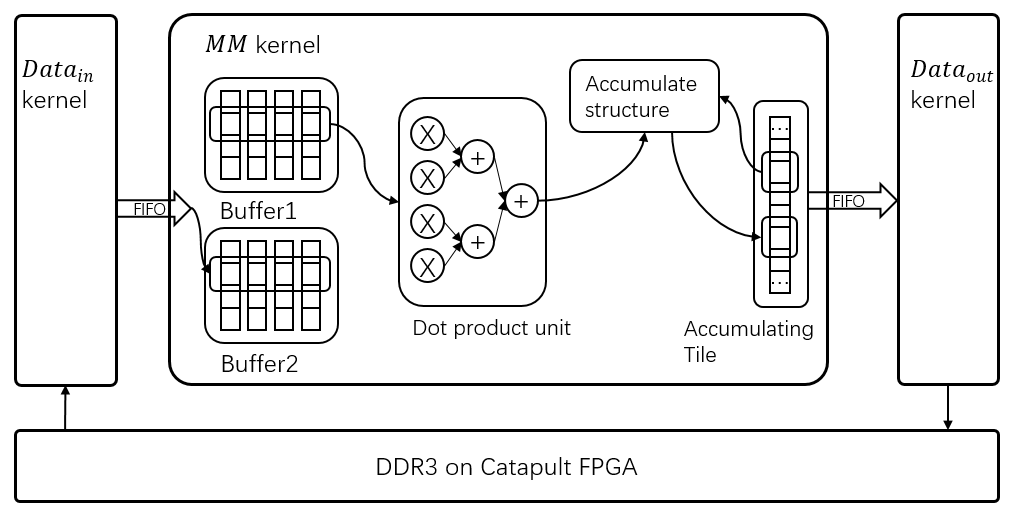
\includegraphics[width=1.0\linewidth]{./figure/z/mm.png}
	\caption{MM kernel}
	\label{mm}
\end{figure}

\subsection{GEMM Specialization Case 1: Convolution Layers}
%The computation performed in convolution layers can be summarized as Equation \ref{conv}. These layers take a set of feature maps as input, and convolve these input with all the trained weights, then output a set of extracted feature maps.
Convolution Layer is the heart of 

\begin{equation}
\centering
Out[x][y][z]=\sum_{i=1}^{N_i}\sum_{j=1}^{K}\sum_{k=1}^{K}In[i][y+i][z+k]*W[x][i][j][k]
\label{conv}
\end{equation}

%To use the $MM$ kernel for the convolution layers, we need to convert the convolution operations into matrix multiplication, and the general strategy for converting a 2d-convolution into MM is provided in Figure \ref{convert}. In this example, there are $M$ input feature maps and $N$ output feature maps. The size of each output feature map is $R\times C$. The size of convolution kernels is $K\times K$, and the sliding stride of convolution is $S$. Here is how we do the converting: First, we partition each output feature map into a single column of the output matrix. To calculate one pixel of one output feature map, we need a patch of input features (size of $K\times K\times M$) and a set of convolution kernels (size of $K\times K\times M$), so we partition a patch of input into a single row of input matrix and the corresponding set of convolution kernels into a single column of weight matrix. All these converting work and data address computing are done in $Data_{in}$ and $Data_{out}$. Once the converting work is done,  we can use our $MM$ kernel to perform convolutions.
%As introduced in Section 3.3, we convert different types of layers into $MM$. The correctness and effectiveness are guaranteed by carefully designed data fetching strategies. However, these data fetching schemes usually need extra operations for address translation, and usually behaves random DRAM accessing, which bring great overhead on data fetching and storing. As a result, we propose to solve this tricky problem by optimizing data layout.
%Here we use a simple example to illustrate the problem and our corresponding optimization. According to Section 3.3, convolution layer performs the most complex convention and data reshaping operations, so we take it for explanation in Figure \ref{datalayout}. We denote the number of input feature maps and size of convolution kernel as $N_{fmap}$ and $K\times K$ respectively. As shown in Figure \ref{datalayout}, we set $N_{fmap}=64$ and $K=2$ in our example. The size of input feature map is 3$\times$3, and the sliding stride of convolution kernel is 1. Conventionally, all input feature maps are stored in DRAM in row-major manner, the detailed storage status is shown in Figure\ref{conventional}. According to Section 3.3 and Section 4.1, we convert the convolution in to matrix multiplication, and perform it in a tiled manner. Here we set the tiling size $S_{tile}=8$. Prior work [cite] usually take advantage of on-line address computing to fetch the proper data for $MM$. Thus, in each row within a tile, there are 8 ($S_{tile}[2][K\times K]$) input features. For the first layer, we illustrate the corresponding DRAM accessing pattern in Figure \ref{conventional}. Unfortunately, this random reading pattern requires recharge for DRAM. Along with the extra address converting computation, the actual bandwidth between DRAM and FPGA chip is restricted to xx GB/s, which makes I/O a critical bottleneck of the overall performance.
%To issue this problem, we optimize the data layout of input feature maps. The result after data layout optimization is generally shown in Figure \ref{datalayout}. For each row within a tile, we reorganize the input features from $S_{tile}[2][K\times K]$ to $S_{tile}[K\times K][2]$. In other words, we packed the features at the same position of each feature map together, and store them in DRAM together to fit the characteristics of sliding convolution kernel. The corresponding DRAM storing status is also shown in Figure \ref{datalayout}. The other input matrix, weight matrix, need to be adjusted accordingly, but the overhead brought by this can be ignored since weights are pre-trained and these adjustments can be applied before model deployment. Thus, with the optimized data layout, the data accessing pattern is in a sequential way, which improves the bandwidth between DRAM and FPGA chip to xx GB/s, and optimizes the bandwidth constraint greatly.  

\begin{figure}
	\centering
	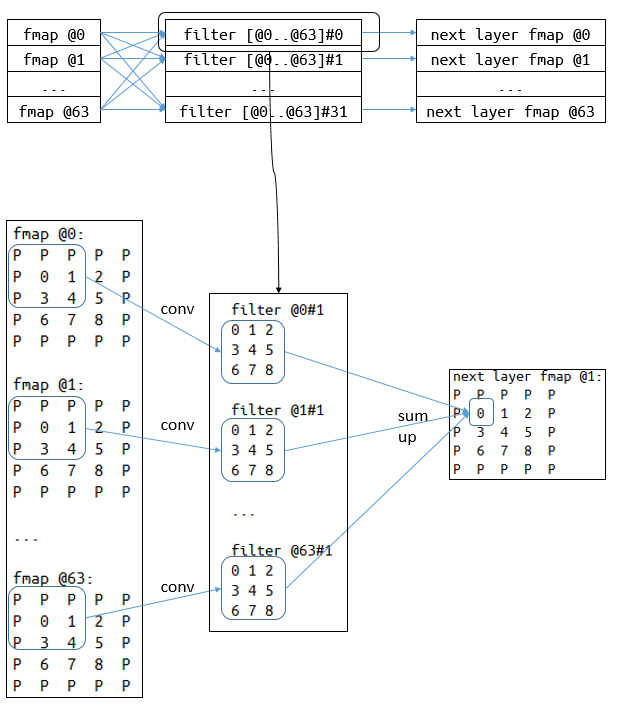
\includegraphics[width=1.0\linewidth]{./figure/z/cnn.png}
	\caption{Convolution Layer}
	\label{cnn}
\end{figure}

Intuitively, for each output element's computing, we need the input elements it concerns to arrive at once. Only in this way can we stream the whole computing, otherwise massive on chip storage are needed of the intermediate results.
Unfortunately, the total input elements that a single output element concerns are widely distributed, both inside a feature map and across feature maps. This could be shown in Figure \ref{cnn}, the computing of every output feature map involves two levels of DDR memory stride: 
1) a single 2-D convolve operation strides across feature map rows.
2) Summing up convolve operation results strids across feature map.
The two level stride leads non-trivial DDR performance problem: Fragmented DDR access wastes DDR burst transfer; Large strided DDR access making DDR frequently recharge. These factors make DDR transfer unable to keep up with computing even with the tiling strategy.
On the other hand, we notice that considerable overlap exists between consecutive filter window sliding. We propose a DDR feature map layout, along with the its corresponding tiling strategy,
that makes our gemm not only fetch from DDR sequencially, but also reuses the consecutive fetched tile.

Our strategy is shown in Figure \ref{layout}, We use $@$ to denote input feature maps, $\#$ to denote filters (also output feature maps).
In our notation,
$5@6$ means the 5th element of the 6th input feature map;
$6@7\#4$ means the 6th element of the 7th subfilter of the 4th filter;
$7\#4$ means the 7th element of the 4th output feature map.
$P$ means padding in the target matrix (padded on the fly in kernel $Data_{in}$).

Suppose our tile A has size of $R_{tile a}$ rows and $L$ columns, we pack the elements at the same position of $L$ feature maps together in DDR storage.
Figure \ref{layout} shows that: Inside a row, $L$ elements lays in sequential; Consecutive rows corresponds to consecutive feature map position, which are also sequential in DDR.
When fetching a tile, we fetch row by row, so the entire fetching of a tile are sequential at DDR.
Also, note that in Figure \ref{layout}, most elements overlaps in three (the filter size in the general case) consecutive tiles, we just need to buffer the previous tile and fetch an extra element to cook up the next tile.
This further saves nearly $(filter\_size - 1)/filter\_size$ DDR transfer.

\begin{figure}
	\centering
	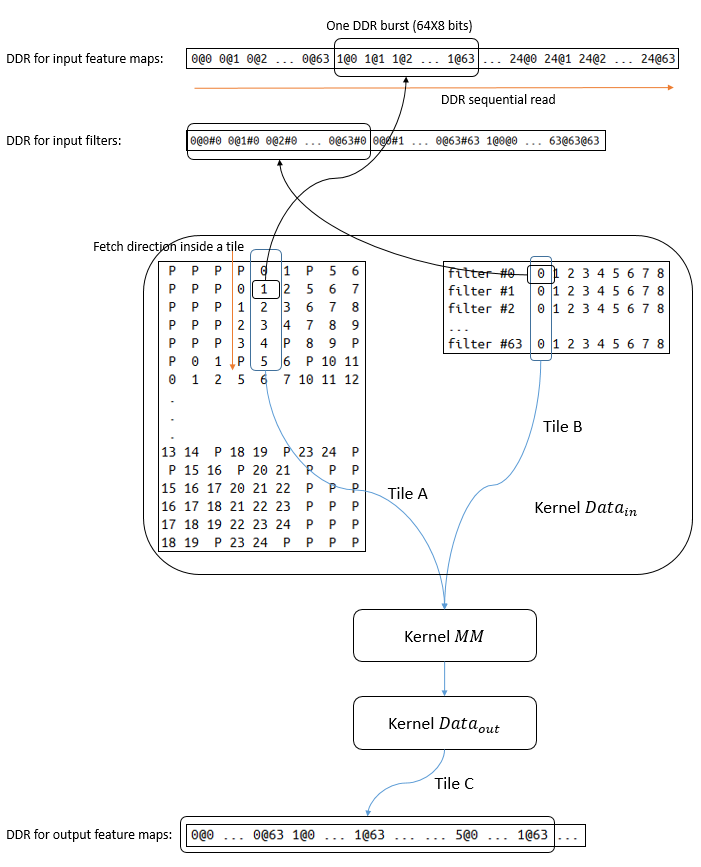
\includegraphics[width=1.0\linewidth]{./figure/z/layout.png}
	\caption{layout}
	\label{layout}
\end{figure}

\subsection{GEMM Specialization Case 2: Recurrent Layers}
In recent years, Long Short-Term Memory (LSTM) has gained great popularity in RNN design. These LSTM-RNNs use LSTM cells in their topological structure, and achieve state-of-art performance in several applications.

\begin{equation}
\centering
\begin{pmatrix}
i\\
f\\
o\\
g\\
\end{pmatrix}
=
\begin{pmatrix}
sigmoid\\
sigmoid\\
sigmoid\\
tanh   \\
\end{pmatrix}
W \times
\begin{pmatrix}
h^{l-1}_t\\
h^{l}_{t-1}\\
\end{pmatrix}
\label{lstmmv}
\end{equation}

\begin{equation}
\centering
c^l_t = f \odot c^l_{t-1} + i \odot g
\label{lstmc}
\end{equation}

\begin{equation}
\centering
h^l_t = o \odot tanh(c^l_t)
\label{lstmh}
\end{equation}

Equation \ref{lstmmv} shows RNN mainly employs $M \times V$ (hidden state vector multiples weight matrix), this operation is inefficient in terms of data locality, for every weight element fetched from DDR is used only once. Recall that ..., we solve this problem by batching $V$ in $M \times V$ as show in \ref{lstmbatch}, every element of $W$ is reused $\#batch$ times.
\[ M \times V \rightarrow M \times (V^1, V^2, \dots, V^{\#batch}) \]
As the mv problem is converted into mm problem, we could reuse our $MM$ kernel.

Besides, several special stratety is took to implement the $Data_out$ kernel template for LSTM application, we take these strategy to explore the specific data flow property in LSTM model.
\begin{itemize}
\item Each gate vector element are used exactly once in element wise operation, $(i_i, f_i, o_i, g_i)$ are used together to update vector $c$ and $h$, this indicates that there is no need to buffer these vectors in $Data_out$. In practice, we arrange these vector as in Figure \ref{lstmvec}, $MM$ kernel outputs $(i_i, f_i, o_i, g_i)$ together and $Data_out$ consumes them immediately.
\item The LSTM model adopts tanh and sigmoid as activation function, these functions are resource-expensive. We notice that activation takes small proportion of the whole computing operations, as could be shown in \ref{lstmmv}, it is $O(N)$ for activation and $O(N^2)$ for $M \times V$. Thus, small amount of activation computing units at kernel $Data_out$ will be enough to keep up with kernel $MM$. In our experiment, we have 1536 vector size V.S. 1024 multipler, one copy of activation function is enough. Taking advantage of this approach, we use fully precision version of sigmoid and tanh instead of interpolation version to promote the model accuracy.
We insert a deep fifo with the capacity of an output tile between kernel $MM$ and kernel $Data_out$, this fifo decomposes the computing process inside two kernels, making both kernels always work at full load asynchronously.
\end{itemize}

\begin{figure}[h]
	\centering
	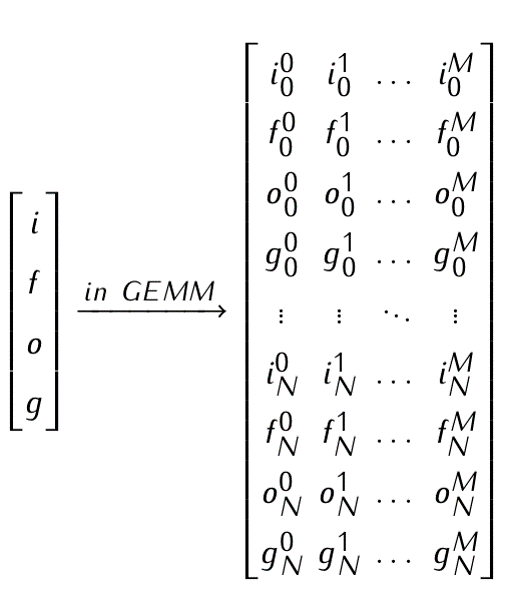
\includegraphics[width=1.0\linewidth]{figure/z/lstmvec.png}
	\caption{Crossed vector layout}
	\label{lstmvec}
\end{figure}



\subsection{Other Layers}
\subsubsection{Fully-Connected Layers}
The computation performed in fully-connected layers can be summarized as Equation \ref{fc}. These layers output a vector ($Out$) as the multiplication of input vector ($In$) and weight matrix ($Weight$).

\begin{equation}
\centering
Out[x]=\sum_{i=1}^{N_i}In[i]\ *\ Weight[x][i]
\label{fc}
\end{equation}

As a result, computation inside fully-connected layers can be viewed as matrix multiplying vector. We reuse our $MM$ kernel to perform it by simply setting column dimension of input matrix B to 1. 


\subsubsection{Pooling Layers}
The operations performed in pooling layers can be summarized as Equation \ref{pooling}
Typically, pooling layers take the maximum (max-pooling) or the average (average-pooling) of the input features in a pooling window as the result to output. Pooling layers are always responsible for sub-sampling features. Though not much opetation involved in, pooling window stride 2-D address space, it is complex to add pooling to $Data_out$ kernel, so we implement separate pooling kernel for flexibility and extensibility.
In this manner, we could reuse our $MM$ kernel.

\begin{equation}
\centering
Out[x]= Pooling_Funcion(x)
\label{conv}
\end{equation}

\subsubsection{Activation Layers}
The operations in activation layers are always element-wise operation, so there is no need to implement an extra kernel for it. We simply add them to $Data_{out}$ kernel before the outputs are written back to DDR. Note that the total number of activating operation is much less than $M\times M$ or $M\times V$ operation, so we put less resource to activation than GEMM without stalling the whole system's pipeline.

\subsection{Performance Estimation}
Before finally deploying deep learning models onto FPGA, model designers may want to have a rough estimation about the performance for model inference. The estimated results are also quite helpful for model designers to improve their designs. As a result, our framework can report an estimated performance of the target deep learning model on FPGA.  

The total number of operations inside a $MM$ kernel can be estimated as  $2\times S_{tile}^3$. The execution time of a $MM$ includes both matrix multiplication and data communication, so the total cycles used for a tile is $S_{tile}^3 \div N_{DSP}$(???).
As a result, we can estimate the performance (in GOPS, giga operations per second)of our $MM$ kernel through Equation \ref{perf}, where $Freq$ indicates the running frequency of FPGA board.

\begin{equation}
\centering
\begin{split}
Performance\ &=\ \dfrac{Operations}{Execution\ Time} \\
&=\ \dfrac{2\times S_{tile}^3}{Cycles/Freq}
\end{split}
\label{perf} 
\end{equation}

Equation \ref{perf} shows that several parameters ($S_{tile}$, $N_{DSP}$,..) can vary in different implementations. Each group of choices for these parameters corresponds to a possible configuration for hardware implementation. Thus, the massive possibilities form a huge design space. So we need to explore the whole design space for the optimal one. This exploration problem can be formulated as follows.
\begin{equation}
\centering
\begin{split}
&Variable:\ Optimization\ parameters???, Frequency \\
&Constraints: Resource (DSP), Bandwidth \\
&Target: Maximum Performance((areto\ Optimality)
\end{split}
\end{equation}
 
This exploration work can be accomplished by simple algorithms for integer programming problems. The $Symbolic\ Compiler$ in our framework can help to explore the design space and  find the optimal hardware configuration. Then it will report the estimated performance and generate the corresponding codes for HLS tools.

\section{Evaluation}
Numerous prior works have shown that deep learning models are robust enough even with a decrease on data precision. Many great works [cite, cite,...] on accelerating deep learning model inference used fixed-point parameters in their design for performance improving and resource saving. Recently, Bengio et.al found that deep CNN models can even use binary values for model inference without much accuracy loss[cite]. So in our implementation, we also support implementing a fixed-point version of the target model. However, the accuracy loss brought by data quantization must be estimated and tested by the model designers in advance, and they need to make a decision on the trade-off between accuracy and performance. 

To illustrate the effectiveness and great performance achieved by our proposed framework, we design and implement three models as our case studies for modern typical deep learning structures: ANN (or feedforward neural network), CNN, and RNN. 


\subsection{Experimental setup}
For the software part, the $Symbolic\ Compiler$ that performs performance estimation, resourse estimation, parameter decision, and OpenCL codes generation is written in Python X.X. To implement our desing on FPGA board, we take advantage of a high-level synthesis design tool, Altera AOCL (vXXX). This high-level synthesis tool help us synthesis and implement the OpenCL-based codes into binary files to program FPGA. The codes on host is written in C++, and compiled by Visual Studio XXX.

For the hardware part, we use a PikesPeak board, with an Altera Stratix-V GSMD5 FPGA on it. An 8GB DDR3 is integrated with the FPGA chip as external storage. The working  frequency of hardware implementation is set to 200MHz. This FPGA board is plugged into a PCI-e slot of a host PC. The CPU inside host is XXXXX, XXGHz,

For performance comparison, we implement software inference on a Xeon CPU. It has XX cores and a XXMB L1 cache. The working frequency of it is xx GHz.

\subsection{Experimental results}

\subsubsection{Performance}
$MM$ kernel is the core part of FPGA-based model inference, so we compared the performance of our $MM$ kernel with other state-of-the-art implementations. We show the performance (in GOPS) of our implementations (floating-point and 8-bit fixed point), Intel MKL[] and Altera MM example design[] in Figure \ref{performance}. Our implementation and Altera MM example design run on the same FPGA board, and Intel MKL runs on the CPU introduced in Section 5.1. From Figure \ref{performance}, we can see that our 32-bit and 8-bit implementations of MM can outperform Intel MKL by XXx and XXx respectively, and the speed-ups on Altera MM example design is XXx and XXx on average.

%\begin{figure}
%	\centering
%	\includegraphics[width=1.0\linewidth]{./figure/performance.jpg}
%	\caption{performance}
%	\label{performance}
%\end{figure}

To show the performance of our framework on a complete model, we compare our CNN implementations with previous accelerators, since there have been massive prior work on it. The comparison results are shown in Table \ref{cnn}.

\begin{table}[h]
	\centering
	\begin{tabular}{|l|c|c|c|}
		\hline
		 & ref & Our Imp & Our Imp \\
		\hline
		FPGA chip & & Stratix-V GSMD5& \\
		\hline
		Frequency & & 200MHz & \\
		\hline
		CNN size & & GOP & \\
		\hline
		Precision & & float(32b) & fixed(8b)\\
		\hline
		Performance & & GFLOPS & GOPS \\
		\hline
	\end{tabular}
	\caption{CNN performance comparison with prior work}
	\label{cnn}
\end{table}

\subsubsection{Energy Efficiency}
To show the great energy efficiency provided by our framework, we compare our implementations with those on CPU and GPU? in Figure \ref{ee}. Several deep learning models are used as benchmarks: DSSM [cite] (ANN), VGG-19 [cite] (CNN), LSTM [cite] (RNN). The energy efficiency is measured in GOPS/W (giga ops per watt). Figure \ref{ee} shows that, in energy efficiency, our framework can outperform CPU by XXx and GPU by XXx on average.  

\begin{figure}
	\centering
	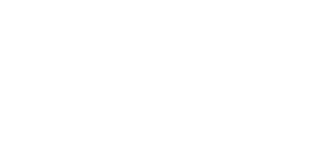
\includegraphics[width=1.0\linewidth]{./figure/blank.jpg}
	\caption{energy efficiency comparison with cpu and gpu}
	\label{ee}
\end{figure}

\subsubsection{Framework Effectiveness}
For all the implemented models in Figure \ref{ee}, our framework meanly takes about 4-5 hours to accomplish the hardware implementation from TensorFlow-described models. While it will take an experienced hardware engineer two weeks to implement one deep learning model on FPGA. So our framework can improve the efficiency of deep learning models' deployment by about 80x. Furthermore, designers with little knowledge about hardware implementation details can also easily use our framework, which indicates that our framework can be widely popularized and benefit the FPGA community.

The accuracy of the estimation models in $Symbolic\ Compiler$ is evaluated in Figure \ref{estimate}. We show the comparison between estimated performance and measured performance of implemented models in Section 5.2.2, and we can see that our proposed models are accurate enough with only XX \% error.

\begin{figure}
	\centering
	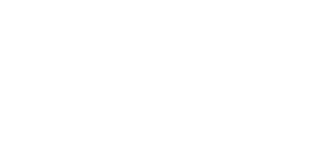
\includegraphics[width=1.0\linewidth]{./figure/blank.jpg}
	\caption{comparison between estimation and measurement}
	\label{estimate}
\end{figure}

%\section{Related work}

\section{Conclusions and future work}
In this paper, we propose a framework that automatically migrates TensorFlow described deep learning models to FPGA implementation for inference acceleration. We also propose several performance models and resource estimations to choose the optimal design configuration. Our case studies show the great performance and effectiveness achieved by this framework.

However, there are still several directions for future research. First, we will go on working with a distributed version of this framework on an FPGA fabric. Second, we will adapt the kernels inside our framework to support emerging optimization techniques for deep learning models like pruning, binarization, etc. Last but not least, we will further extend our framework to model training.


%ACKNOWLEDGMENTS are optional
%\section{Acknowledgments}

%
% The following two commands are all you need in the
% initial runs of your .tex file to
% produce the bibliography for the citations in your paper.
\bibliographystyle{abbrv}
\bibliography{sigproc}  % sigproc.bib is the name of the Bibliography in this case
% You must have a proper ".bib" file
%  and remember to run:
% latex bibtex latex latex
% to resolve all references
%
% ACM needs 'a single self-contained file'!
%

% That's all folks!
\end{document}
